% ##################################################################################################################
\section{Patna}
\label{sec:patna}
\hfill \textbf{Author:} Amit Agarwal

% ##################################################################################################################
Patna is a medium sized city in eastern part of India. Similar to other developing nations, in Patna also, traffic conditions are heterogeneous. There is a high number of bikes and motorbikes (37\,\%, including 4\,\% cycle rickshaws, and 14\,\% respectively). Public transport accounts for 18\,\% and walk for 29\,\%; only 2\,\% of all trips are done by car. Therefore, the \gls{matsim} queue simulation is modified to simulate travel demand under mixed traffic conditions.

The Patna scenario is created using household survey data from a comprehensive mobility plan for Patna \citep[][]{TrippItransVks2009PatnaReport}. To create the Patna scenario, the area under Patna Municipal Corporation is used. The scenario is composed of 72\,zones with a population of about 1.57\,million (year 2008). In this scenario, \gls{matsim} demand is generated using trip diaries. Car, motorbike and bike are used as main congested modes (Figure~\ref{fig:patna0}). Passenger car unit for vehicles is derived using effective area occupied by vehicles. In order to allow overtaking of slower vehicles (bike) by faster vehicles (car and motorbike), preexisting, state-of-the-art \gls{fifo} queue simulation is overridden using earliest link exit time as shown in Figure~\ref{fig:patna1}. 

\ah{make that point clearer - see mail Amit. Possibly extend multi-modal chapter}
\ah{where is code. If in palyground, then describe here. If as contribution, then describe in multi-modal chapter.}

A detailed description of the scenario can be found in \citet[][]{AgarwalEtcMixedTraffic}.

Later, the behavior of traffic ow in modified queue simulation is analyzed by plotting fundamental diagrams and space time trajectories for car, motorbike and bike.

\createfigure%
{Patna: Various vehicles on network, car in red, motorbike in blue and bike in green}%
{Patna: Various vehicles on network, car in red, motorbike in blue and bike in green}%
{\label{fig:patna0}}%
{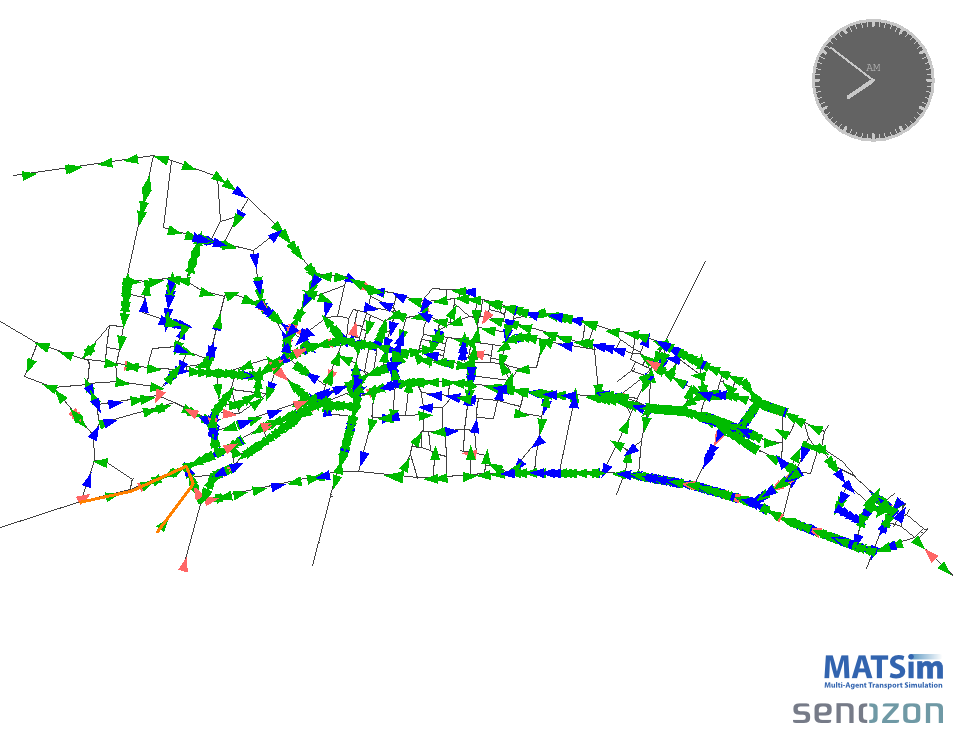
\includegraphics[width=0.99\textwidth, angle=0]{using/figures/vehiclesOnNetwork}}%
{}

\createfigure%
{Patna: \protect\gls{fifo} approach and passing of bicycle by car on a link (not to scale)}%
{Patna: \protect\gls{fifo} approach and passing of bicycle by car on a link (not to scale)}%
{\label{fig:patna1}}%
{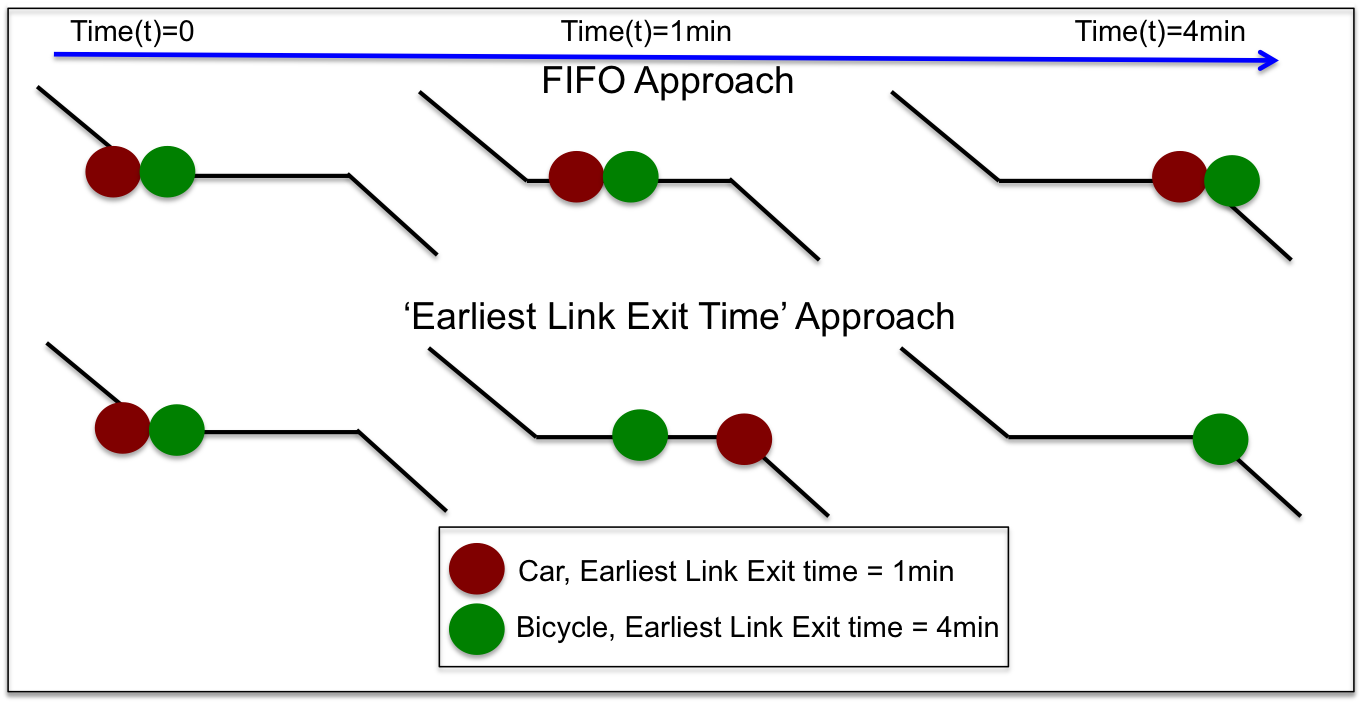
\includegraphics[width=0.99\textwidth, angle=0]{using/figures/FIFOandPassing}}%
{}

% ##################################################################################################################